\documentclass[twoside,11pt]{article}
\showboxdepth3
\showboxbreadth10
\tracingonline1
% Any additional packages needed should be included after jmlr2e.
% Note that jmlr2e.sty includes epsfig, amssymb, natbib and graphicx,
% and defines many common macros, such as 'proof' and 'example'.
%
% It also sets the bibliographystyle to plainnat; for more information on
% natbib citation styles, see the natbib documentation, a copy of which
% is archived at http://www.jmlr.org/format/natbib.pdf

\usepackage{jmlr2e}
\usepackage{hyperref}
%\usepackage{parskip}

% Definitions of handy macros can go here
\newcommand{\dataset}{{\cal D}}
\newcommand{\fracpartial}[2]{\frac{\partial #1}{\partial  #2}}
% Heading arguments are {volume}{year}{pages}{submitted}{published}{author-full-names}

% Short headings should be running head and authors last names
\ShortHeadings{95-845: AAMLP Article}{Redd and Roberts}
\firstpageno{1}

\begin{document}

\title{Heinz 95-845: Predicting Futures Data:\\ A Neural Network Approach}

\author{\name Andrew Redd \email aredd/aredd@andrew.cmu.edu \\
       \addr Heinz College\\
       Carnegie Mellon University\\
       Pittsburgh, PA, United States
       \AND
       \name Alexander Roberts \email adr1/adr1@andrew.cmu.edu \\
       \addr Heinz College\\
       Carnegie Mellon University\\
       Pittsburgh, PA, United States}


\maketitle

\begin{abstract}
  The commodities futures market is used by producers, such as farmers and miners, and manufacturers to hedge,reduce risk, against price changes. Successful prediction of the future value of a good opens a profit opportunity on that future price. This paper discusses methods to predict the future value of one such commodity future, Kansas City Hard Red Wheat (HRW) using Recurrent Neural Networks (RNNs). Hard Red Wheat is grown primarily in Nebraska, Oklahoma, and Kansas. Our methods incorporate Automated Surface Observing Systems (ASOS) weather readings provided by the National Oceanic and Atmosphereic Administration (NOAA) in an effort to improve prediction outcomes.
\end{abstract}

\section{Introduction}

Although many factors influence the future price of HRW wheat in the US, we believe that weather in the region the crop is grown is a significant contributor the market uses in determining the price of the future.  Harsh winter chills can delay the germination of the wheat seed leading to a bad crop and increase in prices while on the other hand temperate weather condusive to wheat growing can lead to an abundant crop yield driving down prices.  The purpose of this paper is to highlight several neural network models that use historic financial data and NOAA ASOS weather readings to predict the price of a wheat future contract 30 days into the future. The majority of literature on modeling financial markets using deep learning methods is proprietary. Of the available literature, all used historic futures contract price movement to predict future movement. Our hypothesis of incorporating weather data to improve on future only data predictions failed to result in improve the model prediction. 

\subsection{Futures Contracts}
The future is risky. Individuals have a heterogeneous perception of future outcomes. This heterogeneity of belief combined with the heterogeneity of risk aversion among individuals creates risk gaps that can be filled contractually. These contracts reduce risk by specifying how both parties will act in the future in regards to supplying and demanding goods. Producers, consumers, and investors are able to speculate on perceived outcomes by contracting to buy or sell an item in the future at a locked-in price. The value of the right to buy at this locked-in price is therefore the market's consensus of the future price of a good given all current publicly available information. A model that can more effectively translate current information into a valid prediction of the future price would enable a speculator to realize larger trading profits.

\subsection{The US Wheat Market}
Wheat is the third most-planted crop in the US. It first began trading on the futures market in 1877. Kansas City Hard Red Winter Wheat is an important component of the US wheat market, being integral for most baking needs. HRW wheat is primarily grown in relatively small geographic area across Oklahoma, Kansas, and Nebraska. (\cite{CME}) As a result, HRW wheat's risk profile with respect to weather factors is relatively less diversified when compared to other commodities. This geographically tight growing area makes HRW a good target for weather-based futures prediction. 

\subsection{Paper Structure}
In Section \ref{background}, we define key topics in futures trading. In Section \ref{model}, we provide a high-level overview of Recurrent Neural Nets (RNNs) and RNN layers such as Long-Short Term Memory (LSTM) and Gated Recurrent Units (GRU). Section \ref{experiment} describes the data sources and data preparation that lead up to the RNN models.  In Section \ref{results}, we discuss the efficiency of our predictions in terms our scoring metric, Mean Squared Error (MSE). 

\section{Background} \label{background}

\subsection{Futures Trading}
	A futures contract is defined as "an agreement to buy or sell an underlying financial instrument or commodity at a specified future date and price." This contract enables producers to hedge risk and speculators to take on risk in relation to a given commodity. (\cite{InvestopediaF})
	
  Producers or a commodity, or manufacturers that depend on a commodity input can use futures to hedge their risk to future price movements. Imagine a wheat farmer, who in anticipation of a bumper, high yielding, year across the Midwest, desires to lock in a price today at which he can sell his crop he will harvest in three months rather than worry about price flucuations.  This allows the farmer to focus on farmer. Further imagine a bread baker, who fears international wheat demand may cause a spike in price in the US wheat market, wishes to lock-in the price of wheat and ensure a supply for his key input. In both cases, the producers are able to hedge away potential price risks using a futures contract to ensure they are able to continue farming and baker.
  
  Speculators in the market are organizations that willing to take on this price risk in hopes of a favorable price change.

  An investor in futures (speculator or producer) is defined to have entered a "long" position if he/she agrees to purchase a good at a specified time and price in the future. An investor is termed to have entered a "short" position if he/she agrees to deliver a good at a specified time and price in the future. If an investor enters a long futures position and the market price goes up \textdollar1 during any daily time period, the investor has the option to purchase a more expensive good at a lower price in the future and thus profits \textdollar 1 per unit covered by the contract. Conversely, if the price of the good drops, the investor loses \textdollar 1 per unit covered by the contract. The opposite case holds true for the short position and market changes held constant.
  
  Futures contracts have two types of settlements. The first type is a cash settlement. This setting involves paying the cash difference between the futures contract price and the spot/market price at the time of contract expiration. The second type is physical delivery which requires the provider of the contract to deliver the actual goods. This applies to commodities such as wheat, oil, energy, and farm animals. The majority of futures contracts are settled via a cash settlement.
  
  Investors often wish to maintain a position (long/short) in a given commodity for a longer period of time than the specified contract duration. In this case the contract is rolled over "by closing the initial contract and opening a new longer-term contract for the same underlying asset at the then-current market price." \cite{InvestopediaRF}

  While many other strategies exist in futures trading, the defined long and short positions provide sufficent context for the motivation behind a better mechanism to predict the futures price.
 
\subsection{Weather's Impact on Wheat}
	
	Wheat quality has many measures such as protein content, grain structure, and grain weight. These quality measures are affected by a variety of variables such as soil quality, grain type, agronomy interventions, and growing climate conditions. Many studies have tried to model these effects in an effort to predict wheat yield within a time horizon to improve yield through intervention. \cite{Gooding2017} found that 70\% of crop variation could be accounted for by wheat type, fertilizer application, and precipitation during the winter and spring. Their model could account 90\% of the annual variation after including summer temperature. Further studies have shown that daily fluctuation measurements are critical to properly predicting wheat outcomes. (\cite{Nuttall2017} \cite{Mearns1996})
	
\subsection{Wheat Price Modeling Assumptions}
We assume that all non observed factors (fertilizer, soil quality, etc) are on average consistent throughout the wheat growing region. This assumption isolates weather as the primary indicator of crop yield and therefore wheat supply. We also assume that future demand is appropriately modeled by the futures price today. The final assumption is that predicted wheat supply is not accounting for all weather-related effects on the wheat crop and therefore wheat supply. These three assumptions isolate the current futures price and the weather as two main drivers of the true future price. 
	

\section{Method: Neural Networks} \label{model}

Since their development in the late 1980s, neural networks have become a mainstay in machine learning. (\cite{Schmidhuber2015}) Recurrent neural networks were designed to handle sequential information through a looping network structure that would pass data inputs to adjacent nodes. (see Figure \ref{fig:unrolledRNN})

\begin{figure}[htbp]
	\centering
	\includegraphics[width=3in]{RNN-unrolled.png}
	\caption{Example of unrolled RNN}
	\label{fig:unrolledRNN}
\end{figure}

Long Short-term memory (LSTM) and Gated Recurrent Units have been researched to further develop the idea of persistence of sequential effect. (\cite{Hochreiter1997}, \cite{Chung}) These methods provide even greater "memory" to the model, enabling networks to better work off of historic data. 

These methods have been used in a myriad of sectors to provide a better prediction where other statistical methods have failed. (\cite{Ugurlu2018}) They have also proven useful in the prediction of stock patterns. (\cite{YoungohcYoon}) 

We use keras to implement a series of models that use Simple RNN, LSTM, and GRU layers. \cite{chollet2015keras}. The implementation code can be found at \url{https://github.com/aredd-cmu/aa-project}

\section{Methods} \label{Methods}

The structure under which we employ these methods is designed to search for the optimal network within our constrained resources. We perform grid search over the number of specialized layers (simple RNN, GRU, LSTM) and different configurations of neurons (see futures\_data.ipynb in code repository). We found that four specialized layers produced the best results over our set with the following set of neurons at each respective layer [256, 256, 128, 32, 16, 1]. We used MSE as the selection criteria.

After selecting the general model hyperparameters we generated a series of models to try to identify the type of specialized layer that may be able to best predict futures outcomes. We used the structure shown in Table \ref{tab:networkstructure} across all methods to isolate the specialized layers in the design.

\begin{table}[htbp]
	\centering
	\begin{tabular}{lclc}
		Layer Type & Output Shape \\
		\hline \\[-11pt]
		Dense & 256 \\
		Spec Layer*(\# of spec. layers-1) & 256\\
		Spec Layer & 128\\
		Dense & 32\\
		Dense & 16\\
		Dense & 1\\
		\hline
	\end{tabular}
	\caption{Abstract network structure example}\label{tab:networkstructure}
\end{table}


We built off the idea of stacking specialized (RNN/GRU/LSTM) layers based on work others have used in prediciting financial outcomes and added the idea of grid searching over the number of specialized layers to stack to find the best model design. (\cite{benjikcf})

\subsection{Data Extraction}

\subsection{Weather Data}
	The Automated Surface Observing System (ASOS) was commissioned in the early 1990s with the intent of modernizing weather reporting in the US. For this project we used an API provided by Iowa State University that outputs daily aggregates of the minute data provided by ASOS. The output variables are listed in Appendix A: Weather Variable List.
	
	\subsubsection{Time Period Selection}
	The API retrieves weather data for a given time period at a given airport. We used a secondary API call to identify all eligible airports in the Kansas, Oklahoma, and Nebraska regions. Even though ASOS was commissioned in the 1990s much of the infrastructure was not in place until the early 2000s. We wanted to explore the trade off between more collection sites and a greater weather history. We determined the optimal time period by evaluating the number of operational stations in the ASOS system by year. We did this by pulling the data for every site across all three states for the years from 1998 - 2018 and received the output in Figure \ref{fig:asosstations}. 
	
	We defined an online station as having the number of rows that corresponded to one of the top three row numbers for the year. This method assumes that the majority of stations are operational with a full dataset and will thus define a "online" data size in number of rows by multiple votes. The year period that we chose was 2005 to 2018.
	
	\textit{NOTE: The anomaly from 2007-2009 seems to be an API issue related to those specific years. We still get data for those years in 2004-2005 periods.}
	
	\begin{figure}[htbp]
		\centering
		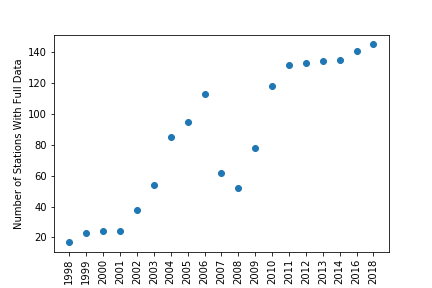
\includegraphics[width=3in]{ASOSstations.png}
		\caption{ASOS Online Stations over Time}
		\label{fig:asosstations}
	\end{figure}

	One concern related to choosing the appropriate time period relative to the number of online stations was that of losing our representative weather spread across the geographic region. We verified that our 2005 decision did not remove more rural stations from the data set by visualizing a map of values across the geographic region shown below in Figure 
	
	\begin{figure}[htbp]
		\centering
		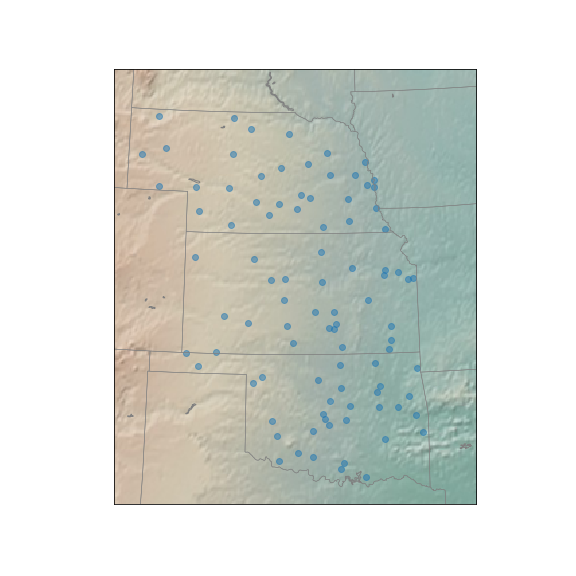
\includegraphics[width=3in]{ASOSspread.png}
		\caption{ASOS Online Stations over Time}\label{fig:asosspread}
	\end{figure}
	
	\subsection{Cleaning Data}
	First, The aggregated data had severe outliers along multiple columns due likely to sensor malfunction. (i.e. Max temperature of 921,613$^oF$) We handled these outliers using the following heuristics found via weather extremes recorded online shown in Table \ref{tab:bounds}. Since the values were large, conventional outlier methods weren't getting the variable ranges down to expected even after method application.  

	\begin{table}[htbp]
		\centering
		\begin{tabular}{ccc}
			Variable & Upper Bound & Lower Bound \\
			\hline \\[-11pt]
			max\_temp\_f & 130 & min(-50, min(min\_temp\_f))\\
			min\_temp\_f & 130 & -50 \\
			max\_dewpoint\_f & 90 & -20\\
			min\_dewpoint\_f & 90 & -20\\
			precip\_in & 70 & 0\\
			\hline
		\end{tabular}
		\caption{List of upper and lower bounds used to clean data outlier observations due to sensor malfunction}\label{tab:bounds}
	\end{table}

	Second, several of the values across the dataset were missing. Assuming that the data was lost because of a weather or geographically related sensor malfunction, we assert that the data is missing at random and impute based on our data values. The data was imputed assuming the variables followed a multivariate normal distribution using the Amelia II implementation in R. (\cite{ameila})
	
	Finally, the data was transformed into wide format in preparation for the merge with the futures data. 

\subsection{Futures Data}
 
We retrieved the futures prices from Quandl API which provides free continuous futures contracts data. Individual futures contracts trade for a finite period of time and continuous futures data 'stitches' together rolling futures contracts to simulate a continous time series of prices.  For example, 3rd-month continuous contract prices use the prices of the 3rd earliest futures contract available which would be the September 2018 contract (as it is April 2018 at the time of this writing).  The raw data form of the output was high, low, close, volume, and adjusted close. We decided to use the 3rd-month continous contract as a it would have less volatility in price due to contract changes (i.e. three months prior to contract termination, the current contract is sold and the next contract period is purchased)

The data output was relatively clean coming out of the CME API. We made minor changes to date and price format to work with our models.

\subsection{Combining and Splitting}

A major decision was made at this step of the data pipeline to only include weather data during days that we had changing futures data (business days when the futures market was open). This decision reduced our weather data sequentiality in exchange for avoiding imputation of weekend values of futures data. Future iterations of this work would cross validate outcomes by using carry forward of pull back imputation to either use Friday or Monday values as proxy for weekend futures data. 

A full picture of our data pipeline is shown in figure \ref{fig:datapipeline}. We continue our discussion of the later end of the data pipeline with the results in section \ref{results}.

\begin{figure}[htbp]
	\centering
	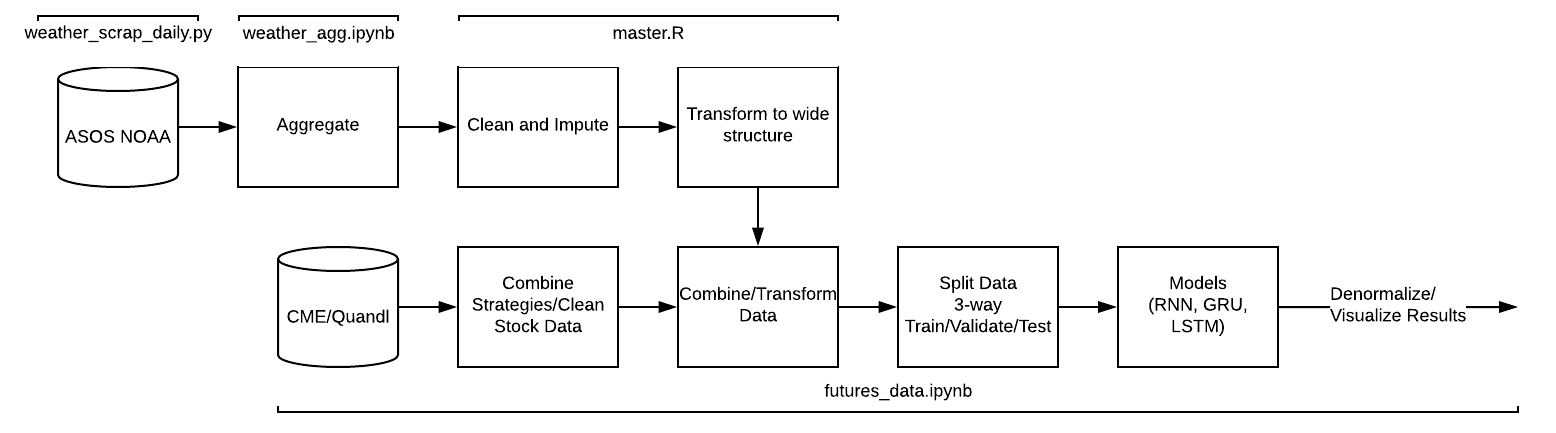
\includegraphics[width=6in]{DataPipeline.png}
	\caption{Data pipeline overview}
	\label{fig:datapipeline}
\end{figure}


\subsection{Feature Choices}

Many traders will use technical analysis in order to capture an ongoing trend in the financial product. We used Open-High-Low-Close (OHLC) average, daily percent change, and 50, 100, and 200 day moving averages in order to communicate such trends.  

In this phase we also transformed our data into a sequence appropriate for an RNN. This sequence involved taking a sliding window along our dataset. The sliding window size we implemented was 44 working days (~ 2 mo.). We then crafted our target as a look-ahead variable 22 working days into the future. The output to this process is a matrix shaped (\# of windows (nrows - window size - look-ahead value), window size, ncols). The sequential nature of the input means that our inputs are no longer i.i.d., but as we are concerned with sequence of events this seems to be appropriate. In our baseline model (feed forward neural net) we do not perform this transformation and assume i.i.d. observations. 

\subsection{Comparison Methods}

In order to validate an improved prediction we take today's closing price and use that as the best prediction for the future closing price. This comparison is on a rolling basis and thus will not equate to the actual future contract final price, but serves a proxy to see how the market already performs  in predicting the price one month out. 

As our comparison methods, we implement a feed-forward (FF) neural network (NN), a fully-connected RNN where the output is to be fed back to input, a gated recurrent unit (GRU) and a long-short term memory (LSTM). The later three NNs being implementations of a recurrent neural network. For each addition of data (futures only, futures and weather, and futures and weather and wheat ETFs) we run the four methods above and compare to the MSE values of our baseline. We anticipated the RNN implementations to outperform FF and baseline. We further anticipated that the addition of more data sources would improve model performance. 

\subsection{Evaluation Criteria}

Since the variable, that we are considering is real valued constrained between zero and one (normalized future price) we use NNs in this context as a regression model. A common error metric is mean squared error (the variance of model residuals). Our definition of a successful model is therefore a model that produces a small variance of error over time. Such a model would likely outperform the model over the long-term. 

\section{Results} \label{results}

\subsection{Futures Only}

The subset of models that involved only futures data were high performers in our experiments. The baseline carry forward for this subset of data was 0.0014. The results of each model is shown in Table \ref{tab:futuresonly}.

\begin{table}[h!]
	\begin{center}
		\begin{tabular}{ccc}
		    Method & Train MSE & Test MSE \\
		\hline \\[-11pt]
		Feed-Forward & 0.000005 & 0.000039 \\
		Simple RNN & 0.007647 & 0.097884 \\ 
	    GRU & 0.018110 & 0.160860 \\
		LSTM & 0.017986 & 0.160441 \\
		\hline
		\end{tabular}
		\caption{Training and testing MSE of neural network types over futures only data}\label{tab:futuresonly}
	\end{center}
\end{table}

The feed-forward network had very high precision and beat the baseline over the same period. However, the RNN implementations failed to beat the baseline and under LSTM and GRU implementations the test MSE was lower than the train MSE. We attributed this very non-intuitive result to the high variance of the futures price in our training set and the relatively low volatility in our test set. This is visualized in figure \ref{fig:futuresonlygraph}. 

\begin{figure}[htbp]
	\centering
	\includegraphics[width=5in]{futuresonlygraph.png}
	\caption{Model confusion over major spikes in futures price. These spikes occured more in the training period (pre-October 1990)} \label{fig:futuresonlygraph}
\end{figure}

We note that the model is not able to adequately account for the extreme spikes in the futures price. As a result the model would perform better during times of relatively low variance throughout the market. While finding is not surprising, it underscores the difficulty of predicting the face of unanticipated increases and decreases in the market.   

\subsection{Futures and Weather}

These models incorporated both futures and weather data beginning in 2005. We also ran the futures only data over the same period as an additional baseline. We intuitively anticipated that the addition of more data would add greater richness to the prediction. The baseline MSE for this time period is 0.0034. The results are shown in table \ref{tab:futuresandweather}.

\begin{table}[h!]
	\begin{center}
		\begin{tabular}{ccc}
			Method & Train MSE & Test MSE \\
			\hline \\[-11pt]
			Feed-Forward & 0.000889 & 0.000260 \\
			Simple RNN & 0.222644 & 0.118933 \\ 
			GRU & 0.197310 & 0.096303 \\
			LSTM & 0.204753 & 0.100222 \\
			\hline
		\end{tabular}
	\quad
		\begin{tabular}{ccc}
			Train MSE & Test MSE \\
			\hline \\[-11pt]
			0.012446 & 0.005717 \\
			0.167684 & 0.075022 \\ 
			0.217229 & 0.109365 \\
			0.204472 & 0.100299 \\
			\hline
		\end{tabular}
		
		\caption{Training and testing MSE for futures only (left) and futures and weather (right) of neural network types over the same time period}\label{tab:futuresandweather}
	\end{center}
\end{table}

We found that not only were the results worse as a result of introducing the weather data but also the test/train inversion persisted during this time period as well.

%This is a problem because the weather data doesn't go back that far so it is likely something else. We need a graph of this. 

\subsection{Futures, Weather, and Wheat-Related ETFs}

These models are on data ETFs that began in 2011. The test/train period division is October 30, 2013. The baseline prediction MSE over this time period is 0.002. We include the wheat based ETFs as a means to test whether companies' stock in the wheat industry have predictive power in indicating the future price. The results over this time period are show in table \ref{tab:futuresweatherandetf}.

\begin{table}[h!]
		\begin{tabular}{ccc}
			Method & Train MSE & Test MSE \\
			\hline \\[-11pt]
			FF& 0.002405 & 0.003373 \\
			RNN & 0.168831 & 0.033897 \\ 
			GRU & 0.205864 & 0.052294 \\
			LSTM & 0.207230 & 0.052323 \\
			\hline
		\end{tabular}
		\begin{tabular}{ccc}
			Train MSE & Test MSE \\
			\hline \\[-11pt]
			0.014837 & 0.053937 \\
			0.293548 & 0.101416 \\ 
			0.187421 & 0.042839 \\
			0.208780 & 0.053252 \\
			\hline
		\end{tabular}
			\begin{tabular}{ccc}
		Train MSE & Test MSE \\
		\hline \\[-11pt]
		0.016946 & 0.070487 \\
		0.187846 & 0.043364 \\ 
		0.186825 & 0.042947 \\
		0.202720 & 0.050137 \\
		\hline
	\end{tabular}
		
		\caption{Training and testing MSE for futures only (left), futures and weather (middle) and futures, weather and ETF (right) over same time period trained on pre-October 30, 2013}\label{tab:futuresweatherandetf}
\end{table}

We anticipated that given the output of the weather-included forcast, the addition of more variables together with a shorter time frame would likely not improve predictive score. The introduction of the additional variables didn't seem to harm the predictive outcomes, but didn't improve the values at significant levels. 

\section{Conclusion}

In this paper, we reviewed basic concepts within the futures market and developed an intuitive model under which we would be able to forecast the futures contract price. We find the results of this particular forecast to be discouraging to the idea that one can predict futures prices. 

If we had to pursue a model that would best predict the price 22 working days in advance, our results indicate a feed-forward network would be most adept at training and testing on such values. 

In addition to a model suggestion, we have several other observations of note:

\begin{enumerate}
	\item Market Information - The markets are using orders of magnitude more information to arrive at the future price than could be contained in a single model. This fact seems allegorically comparable to the successes of ensemble methods with each actor in the market (though potentially a 'dumb learner') introducing information into the market and yielding a superior prediction. 
	\item Magic Bullets - While very adept at prediction, neural networks take a great deal of precision and iteration in order to produce robust results. This observation strengthens the idea that there is no panacea to every type of prediction.
	\item Further Parameter Tuning - While there are infinite parameter sets to each model, it is important to identify early in model development, key hyperparameters. These parameters are often not in your model.  As a part of further work, we would like to explore tuning window size and look ahead values. 
\end{enumerate}



Summarize your work one more time, this time assuming the reader has read your paper.
Build suspense for what your next extension to this method would be.

% ACKNOWLEDGEMENTS
% \acks{Many thanks to all collaborators and funders!}

\bibliography{project_bib}

\appendix
\section*{Appendix A.}\label{append}
\subsection*{Weather Variable List} \label{weavarlist}
\begin{itemize}
	\item station - Common identifier for the station.
	\item day - Calendar date of the summary.
	\item max\_temp\_f - Maximum Air Temperature [F].
	\item min\_temp\_f - Minimum Air Temperature [F].
	\item max\_dewpoint\_f - Maximum Dew Point [F].
	\item min\_dewpoint\_f - Minimum Dew Point [F].
	\item precip\_in - Daily Precipitation [inch].
	\item avg\_wind\_speed\_kts - Average Wind Speed [knots]
	\item avg\_wind\_drct - Average Wind Direction [deg]
	\item min\_rh - Minimum Relative Humidity [%]
	\item avg\_rh - Average Relative Humidity [%]: computed by time averaging the available reports, it is not average of the daily max\min.
	\item max\_rh - Maximum Relative Humidity [%]
	\item climo\_high\_f - NCDC 1981-2010 Daily High Temperature Climatology [F]
	\item climo\_low\_f - NCDC 1981-2010 Daily Low Temperature Climatology [F]
	\item climo\_precip\_in - NCDC 1981-2010 Daily Precipitation Climatology [inch]
	\item snow\_in - Reported Snowfall [inch]
	\item snowd\_in - Reported Snow Depth [inch]
\end{itemize}

\end{document}
